\documentclass{article}
\usepackage[utf8]{inputenc}
\usepackage[T1]{fontenc}
\usepackage{amsmath, amssymb, amsthm, mathtools, hyperref, enumitem, booktabs}
\usepackage[margin=1in]{geometry}
\usepackage{tikz}
\usetikzlibrary{arrows.meta, positioning, calc}
\usepackage[most]{tcolorbox}
\newtcolorbox{pitfall}[1][]{colback=red!2, colframe=red!45!black,
    fonttitle=\bfseries, coltitle=red!45!black, colbacktitle=red!2, title={Pitfall: #1},
    sharp corners, boxrule=0.6pt, left=6pt, right=6pt, top=4pt, bottom=4pt}

\newtheorem{proposition}{Proposition}
\newtheorem{corollary}[proposition]{Corollary}
\newtheorem{theorem}[proposition]{Theorem}
\newtheorem{lemma}[proposition]{Lemma}
\theoremstyle{definition}
\newtheorem{definition}[proposition]{Definition}
\newtheorem{condition}[proposition]{Condition}
\theoremstyle{remark}
\newtheorem{remark}[proposition]{Remark}
\newtheorem{example}[proposition]{Example}

\title{Causal Modeling Framework}
\author{}
\date{}

\begin{document}
\maketitle

\begin{abstract}
\end{abstract}

\newpage
\section{The Transition Operator}
\label{transitionoperator}

\paragraph{Setting.} We keep the setting of the reference document's sections on Transition Independence and on Sufficient Context and Context Bases, naming rather than re-deriving what is established there: a function $f \colon S_1 \times \cdots \times S_n \to T$ on the total product of the factor sets, which carry no assumed structure; a fixed coordinate $i$; the indices partitioned as $\{i\} \cup J \cup K$, with $J$ the context and $K$ the remaining variables; and $\boldsymbol{a}|_{a_i = a_i'}$ for the tuple identical to $\boldsymbol{a}$ except that its $i$-th component is replaced by $a_i'$. The variable $s_i$ is \textit{transition-independent of $\boldsymbol{s}_K$ given context $\boldsymbol{s}_J$} with respect to $f$ iff there exists a \textit{transition map} $H_{i,J} \colon \mathcal{D}_i^J \times S_i \to T$ (necessarily unique on its declared domain) such that
\begin{equation}
\label{contexttransitionmap}
\forall\, \boldsymbol{a} \in S_1 \times \cdots \times S_n,\;\; \forall\, a_i' \in S_i \quad
f(\boldsymbol{a}|_{a_i = a_i'}) = H_{i,J}\bigl(f(\boldsymbol{a}),\, a_i,\, a_i',\, \boldsymbol{a}_J\bigr),
\end{equation}
where $\mathcal{D}_i^J \coloneqq \{(f(\boldsymbol{a}),\, a_i,\, \boldsymbol{a}_J) : \boldsymbol{a} \in S_1 \times \cdots \times S_n\}$. That section records (\ref{contexttransitionmap}) as equivalent to the following condition, restated here because the existence of this section's object is exactly it.

\begin{remark}[Output-determinacy on context $J$]
\label{contextoutputdeterminacy}
For every $\boldsymbol{a}, \boldsymbol{b} \in S_1 \times \cdots \times S_n$, if $f(\boldsymbol{a}) = f(\boldsymbol{b})$, $a_i = b_i$, and $\boldsymbol{a}_J = \boldsymbol{b}_J$, then $f(\boldsymbol{a}|_{a_i = a_i'}) = f(\boldsymbol{b}|_{b_i = a_i'})$ for every $a_i' \in S_i$.
\end{remark}

\noindent For a value $a_i \in S_i$ and a context tuple $\boldsymbol{a}_J \in \prod_{j \in J} S_j$ we write
\[
f|_{a_i, \boldsymbol{a}_J} \coloneqq f|_{s_i = a_i,\; \boldsymbol{s}_J = \boldsymbol{a}_J} \colon \prod_{m \in K} S_m \to T
\]
for the partial function with the moved coordinate held at $a_i$ and the context held at $\boldsymbol{a}_J$ --- the two values written in the order the operator's bracket will carry them --- and
\[
\mathcal{D}_i^J(a_i,\, \boldsymbol{a}_J) \coloneqq \{v \in T : (v,\, a_i,\, \boldsymbol{a}_J) \in \mathcal{D}_i^J\} \subseteq T
\]
for the fibre of $\mathcal{D}_i^J$ over $(a_i, \boldsymbol{a}_J)$, which is the range of $f|_{a_i, \boldsymbol{a}_J}$: the outputs realized by the tuples carrying $a_i$ at the $i$-th coordinate and $\boldsymbol{a}_J$ on the context. No fibre is empty, and the total product is what makes that so: a value of $S_i$ and a context tuple are chosen independently of each other and of the remaining coordinates, so some tuple carries both. The domain of $f$ is the total product throughout; the strata partition it and nothing is removed from it.

\paragraph{The transition operator.} The section on Sufficient Context and Context Bases reads (\ref{contexttransitionmap}) with the tuple free and reads off a value; this section reads it with the from-value, the target and the context values fixed, and reads off a map.

\begin{definition}[Transition operator]
\label{operatordef}
Let $a_i, a_i' \in S_i$ and $\boldsymbol{a}_J \in \prod_{j \in J} S_j$. A \textit{transition operator} at that triple is a map $\mathsf{T}_{i,J}[a_i, a_i', \boldsymbol{a}_J] \colon \mathcal{D}_i^J(a_i, \boldsymbol{a}_J) \to T$ (necessarily unique on its declared domain, and carrying the target $a_i'$ before the context $\boldsymbol{a}_J$ as $H_{i,J}$ does) such that
\begin{equation}
\label{operatordefining}
\mathsf{T}_{i,J}[a_i,\, a_i',\, \boldsymbol{a}_J] \circ f|_{a_i, \boldsymbol{a}_J} \;=\; f|_{a_i', \boldsymbol{a}_J},
\end{equation}
an equality of maps $\prod_{m \in K} S_m \to T$.
\end{definition}

\noindent Both sides of (\ref{operatordefining}) are functions on $\prod_{m \in K} S_m$: the operator is post-composed with the stratum at the from-value and returns the stratum at the target, the context fixed on both sides and the coordinates $\boldsymbol{s}_K$ untouched. Unfolded at a tuple $\boldsymbol{b}$ carrying $a_i$ at the $i$-th coordinate and $\boldsymbol{a}_J$ on the context, (\ref{operatordefining}) says $\mathsf{T}_{i,J}[a_i, a_i', \boldsymbol{a}_J]\bigl(f(\boldsymbol{b})\bigr) = f(\boldsymbol{b}|_{b_i = a_i'})$, which is (\ref{contexttransitionmap}) with the output moved out of the argument list; the composite on the left is defined because the range of the stratum is exactly $\mathcal{D}_i^J(a_i, \boldsymbol{a}_J)$. Equivalently $\mathsf{T}_{i,J}[a_i, a_i', \boldsymbol{a}_J] = H_{i,J}(\,\cdot\,,\, a_i,\, a_i',\, \boldsymbol{a}_J)$: the operator is the transition map with its three value-level arguments fixed and its output argument left free, and the same equation read from right to left recovers the map from the family. The family and the map are the same data, differently indexed; what changes is what is held fixed. Setting $J = \emptyset$ leaves the context entry the empty tuple, and we drop it together with the second subscript, writing $\mathsf{T}_i[a_i, a_i']$.

\noindent The bracket carries values, not indices: the two coordinate values between which $s_i$ moves, and the context values the operator consults, matching $H_{i,J}(f(\boldsymbol{a}), a_i, a_i', \boldsymbol{a}_J)$ argument for argument, while the subscripts record which coordinate moves and which coordinates the operator is permitted to consult, neither of which the bracket carries. The bracket is an index and the parentheses are application, so $\mathsf{T}_{i,J}[a_i, a_i', \boldsymbol{a}_J]$ is a map before it meets any value. The operator and the transition map carry the same information and differ in what is eaten: $H_{i,J}$ takes the output and returns a value, while $\mathsf{T}_{i,J}[a_i, a_i', \boldsymbol{a}_J]$ takes nothing further and is itself a map on outputs, so it composes with $f$ and with other operators. The non-trivial content of (\ref{operatordefining}) is inherited unchanged from (\ref{contexttransitionmap}), and it is that one map serves every tuple of the stratum at once: the operator post-composes with $f$, so the tuple it is applied at reaches it only through the output, and the coordinates $\boldsymbol{b}_K$ are dropped in favor of that output.

\begin{remark}[Well-definedness]
\label{operatorwelldefined}
A family of maps $\mathsf{T}_{i,J}[a_i, a_i', \boldsymbol{a}_J] \colon \mathcal{D}_i^J(a_i, \boldsymbol{a}_J) \to T$ satisfying (\ref{operatordefining}) at every triple exists iff output-determinacy on context $J$ (Remark~\ref{contextoutputdeterminacy}) holds, and it is then unique.
\end{remark}

\noindent \textit{Proof of the equivalence.} ($\Rightarrow$) Suppose such a family exists, and let $f(\boldsymbol{a}) = f(\boldsymbol{b})$ with $a_i = b_i$ and $\boldsymbol{a}_J = \boldsymbol{b}_J$. Both $\boldsymbol{a}_K$ and $\boldsymbol{b}_K$ lie in the domain of the stratum $f|_{a_i, \boldsymbol{a}_J}$, so (\ref{operatordefining}) evaluated at each gives $f(\boldsymbol{a}|_{a_i = a_i'}) = \mathsf{T}_{i,J}[a_i, a_i', \boldsymbol{a}_J]\bigl(f(\boldsymbol{a})\bigr) = \mathsf{T}_{i,J}[a_i, a_i', \boldsymbol{a}_J]\bigl(f(\boldsymbol{b})\bigr) = f(\boldsymbol{b}|_{b_i = a_i'})$ for every $a_i' \in S_i$. ($\Leftarrow$) Given output-determinacy on context $J$ and $v \in \mathcal{D}_i^J(a_i, \boldsymbol{a}_J)$, set $\mathsf{T}_{i,J}[a_i, a_i', \boldsymbol{a}_J](v) := f(\boldsymbol{a}|_{a_i = a_i'})$ for any $\boldsymbol{a}$ with $f(\boldsymbol{a}) = v$ carrying $a_i$ at the $i$-th coordinate and $\boldsymbol{a}_J$ on the context; output-determinacy on context $J$ makes the choice of $\boldsymbol{a}$ immaterial, so the map is well-defined and (\ref{operatordefining}) holds by construction. Uniqueness follows from (\ref{operatordefining}) alone: every element of $\mathcal{D}_i^J(a_i, \boldsymbol{a}_J)$ is $f|_{a_i, \boldsymbol{a}_J}(\boldsymbol{a}_K)$ for some $\boldsymbol{a}_K$, so every value of the operator is forced.

\noindent Existence at one triple is the weaker demand, and the two are separated below. For $\mathsf{T}_{i,J}[a_i, a_i', \boldsymbol{a}_J]$ to be well-defined on its declared domain it is necessary and sufficient that any two tuples of the stratum sharing an output respond identically to each other under the substitution of $a_i'$: the assignment $f(\boldsymbol{b}) \mapsto f(\boldsymbol{b}|_{b_i = a_i'})$ has all of $\mathcal{D}_i^J(a_i, \boldsymbol{a}_J)$ for its domain by construction and is single-valued exactly then. Quantified over every triple that requirement is Remark~\ref{contextoutputdeterminacy}, which by item (a) of the section on Sufficient Context and Context Bases is (\ref{contexttransitionmap}) itself; asked at one triple it is less, and a mechanism can meet it at some triples and fail it at others. The question is monotone in the context: output-determinacy on context $J$ gives output-determinacy on every larger context, so the contexts carrying the family are closed upward, and how far $J$ can be cut asks where that closure stops rather than whether it stops anywhere.

\paragraph{Relation to the descended transform map.} The reference document's section on Transform Independence writes the transform-map condition as the intertwining identity $f \circ \hat{\delta}_i = \rho(\delta_i) \circ f$, with $\delta_i$ a transform of $S_i$, $\delta_i \ast a_i$ its application, $\hat{\delta}_i$ the map $\boldsymbol{a} \mapsto \boldsymbol{a}|_{a_i = \delta_i \ast a_i}$ it induces on tuples, and $\rho(\delta_i)$ the self-map of the range of $f$ that $\hat{\delta}_i$ descends to, and names the standard objects there: $f$ a semiconjugacy, or factor map, onto its image, and the descent along $f$ the deterministic lumpability of the level-set partition, also known as exact aggregation. The transition operator is the transition-map analogue of that lift, and (\ref{operatordefining}) is the same intertwining read with the substitution of $a_i'$ for $a_i$ in place of a transform, on the tuples carrying $a_i$ and $\boldsymbol{a}_J$ in place of the whole domain, and with $\mathsf{T}_{i,J}$ in place of $\rho$; that material is not repeated here. The two lifts differ in the shape of their declared domains, and the difference is forced by the two conditions rather than chosen. On the transform side the declared domain is a product of the range of $f$ with the family of transforms, the transform being chosen independently of the tuple, so $\rho(\delta_i)$ is a self-map of the whole range and the identity holds at every tuple; on the transition side $\mathcal{D}_i^J$ is not a product, the output and the from-value and the context values constraining each other, so $\mathsf{T}_{i,J}[a_i, a_i', \boldsymbol{a}_J]$ is defined on one fibre and (\ref{operatordefining}) is available at the tuples carrying $a_i$ and $\boldsymbol{a}_J$ and not at the others. What separates the two is the from-value: $\rho$ consults the transform alone while $\mathsf{T}_{i,J}$ consults the pair of values, which is the comparison the reference document draws in the remark on keeping the initial value. The algebra separates with it, and Proposition~\ref{operatorlaws} is where that shows: $\rho$ extends to an action of the closure of the transform family on the range of $f$, a semigroup with no inverses assumed, whereas the transition operators at a fixed context tuple are invertible.

\begin{proposition}[Operator laws]
\label{operatorlaws}
Suppose $s_i$ is transition-independent of $\boldsymbol{s}_K$ given context $\boldsymbol{s}_J$ with respect to $f$, fix a context tuple $\boldsymbol{a}_J$, and let $a_i, a_i', a_i'' \in S_i$. Then $\mathsf{T}_{i,J}[a_i, a_i', \boldsymbol{a}_J]$ carries $\mathcal{D}_i^J(a_i, \boldsymbol{a}_J)$ onto $\mathcal{D}_i^J(a_i', \boldsymbol{a}_J)$, and
\[
\mathsf{T}_{i,J}[a_i',\, a_i'',\, \boldsymbol{a}_J] \circ \mathsf{T}_{i,J}[a_i,\, a_i',\, \boldsymbol{a}_J] = \mathsf{T}_{i,J}[a_i,\, a_i'',\, \boldsymbol{a}_J],
\qquad
\mathsf{T}_{i,J}[a_i,\, a_i,\, \boldsymbol{a}_J] = \mathrm{id},
\]
the first as maps on $\mathcal{D}_i^J(a_i, \boldsymbol{a}_J)$ and the second as the identity map of $\mathcal{D}_i^J(a_i, \boldsymbol{a}_J)$. Consequently $\mathsf{T}_{i,J}[a_i, a_i', \boldsymbol{a}_J]$ is a bijection of $\mathcal{D}_i^J(a_i, \boldsymbol{a}_J)$ onto $\mathcal{D}_i^J(a_i', \boldsymbol{a}_J)$, with inverse $\mathsf{T}_{i,J}[a_i', a_i, \boldsymbol{a}_J]$.
\end{proposition}

\noindent \textit{Proof.} Let $v = f(\boldsymbol{b})$ lie in $\mathcal{D}_i^J(a_i, \boldsymbol{a}_J)$, realized by $\boldsymbol{b}$ with $b_i = a_i$ and $\boldsymbol{b}_J = \boldsymbol{a}_J$, and write $\boldsymbol{b}' \coloneqq \boldsymbol{b}|_{b_i = a_i'}$. Since $i \notin J$, the tuple $\boldsymbol{b}'$ carries $a_i'$ at the $i$-th coordinate and still carries $\boldsymbol{a}_J$ on the context: the substitution moves the coordinate and leaves the context where it stood. Hence $\mathsf{T}_{i,J}[a_i, a_i', \boldsymbol{a}_J](v) = f(\boldsymbol{b}')$ lies in $\mathcal{D}_i^J(a_i', \boldsymbol{a}_J)$, which is the transport claim and is also what makes the composite well-defined; every value of that fibre is reached, being $f(\boldsymbol{c})$ for some $\boldsymbol{c}$ carrying $a_i'$ and $\boldsymbol{a}_J$, hence the image of $f(\boldsymbol{c}|_{c_i = a_i}) \in \mathcal{D}_i^J(a_i, \boldsymbol{a}_J)$. Applying (\ref{operatordefining}) to $\boldsymbol{b}'$ gives
\[
\mathsf{T}_{i,J}[a_i',\, a_i'',\, \boldsymbol{a}_J]\bigl(f(\boldsymbol{b}')\bigr)
= f\bigl((\boldsymbol{b}|_{b_i = a_i'})|_{b_i = a_i''}\bigr)
= f\bigl(\boldsymbol{b}|_{b_i = a_i''}\bigr)
= \mathsf{T}_{i,J}[a_i,\, a_i'',\, \boldsymbol{a}_J](v),
\]
the middle equality because substituting at the $i$-th coordinate twice leaves the value last substituted and nothing of the first. The identity clause is $\boldsymbol{b}|_{b_i = a_i} = \boldsymbol{b}$. For the last claim, the two clauses together give $\mathsf{T}_{i,J}[a_i', a_i, \boldsymbol{a}_J] \circ \mathsf{T}_{i,J}[a_i, a_i', \boldsymbol{a}_J] = \mathrm{id}$ on $\mathcal{D}_i^J(a_i, \boldsymbol{a}_J)$ and, with the two values exchanged, $\mathsf{T}_{i,J}[a_i, a_i', \boldsymbol{a}_J] \circ \mathsf{T}_{i,J}[a_i', a_i, \boldsymbol{a}_J] = \mathrm{id}$ on $\mathcal{D}_i^J(a_i', \boldsymbol{a}_J)$; two maps whose composites in both orders are identities are mutually inverse bijections.

\noindent Read as a diagram, the two clauses are exactly functoriality on the pair groupoid of $S_i$ --- one arrow for each ordered pair of values, composing by $(a_i', a_i'') \circ (a_i, a_i') = (a_i, a_i'')$, with the identity at each value --- so at a fixed context tuple the fibres carry an action of that groupoid, and the invertibility above is the groupoid's rather than a further demand on $f$. The fibres over one context tuple are therefore in bijection with one another. The laws are laws at one context tuple: an operator carried by another context tuple has another declared domain, and the composite across two of them is not declared. The composition law is also not the composition of nested substitutions in distinct coordinates: it is the absorption of successive substitutions in the one coordinate $i$, read downstream of $f$. Of the clauses, the identity one alone is free of the hypothesis --- at a triple whose from-value and target agree the substituted tuple is $\boldsymbol{b}$ itself, so the assignment the operator must carry out is the identity relation on the fibre, single-valued whatever $f$ may be --- and the bijectivity clause is not free: an operator surviving at a single triple where the family fails need not be injective.

\paragraph{The familiar picture.} A causal graph is drawn with a node for each variable and an arrow into a node from each variable its mechanism consults. Take such a drawing, and circle one arrow:
\[
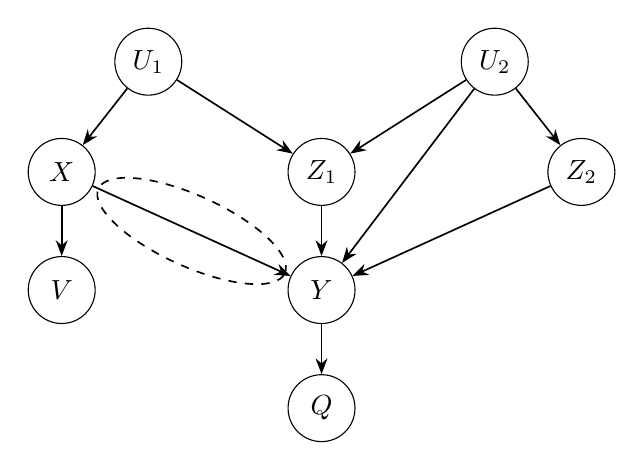
\begin{tikzpicture}[
  vertex/.style={draw, circle, minimum size=8.5mm, inner sep=0pt},
  arc/.style={-{Stealth[length=2mm]}, semithick}]
  \node[vertex] (u1) at (0,3)      {$U_1$};
  \node[vertex] (u2) at (4.4,3)    {$U_2$};
  \node[vertex] (x)  at (-1.1,1.6) {$X$};
  \node[vertex] (z1) at (2.2,1.6)  {$Z_1$};
  \node[vertex] (z2) at (5.5,1.6)  {$Z_2$};
  \node[vertex] (v)  at (-1.1,0.1) {$V$};
  \node[vertex] (y)  at (2.2,0.1)  {$Y$};
  \node[vertex] (q)  at (2.2,-1.4) {$Q$};
  \draw[arc] (u1) -- (x);
  \draw[arc] (u1) -- (z1);
  \draw[arc] (u2) -- (z1);
  \draw[arc] (u2) -- (z2);
  \draw[arc] (u2) -- (y);
  \draw[arc] (z1) -- (y);
  \draw[arc] (z2) -- (y);
  \draw[arc] (x)  -- (v);
  \draw[arc] (x)  -- (y);
  \draw[arc] (y)  -- (q);
  \draw[dashed, semithick, rotate around={-24.4:($(x)!0.5!(y)$)}] ($(x)!0.5!(y)$) ellipse [x radius=13mm, y radius=4.5mm];
\end{tikzpicture}
\]
Read the mechanism at $Y$ as the $f$ above: the variables entering $Y$ supply the coordinates, their value sets supply the factor sets, $T$ is the value set of $Y$, and the source of the circled arrow supplies the coordinate $i$, the remaining arrows into $Y$ supplying the remaining coordinates, from among which the context is drawn. The total product is what the structural reading requires rather than a simplification of it: a mechanism must return a value at every combination of its arguments for the setting of those arguments to be defined at all. What the arrows upstream of $Y$ govern is which tuples the system visits, which is a statement about the system and not about $f$; among the coordinates of $f$ there is no graph, and the drawing carries arrows between two of them here without ordering them or making one of them move another, contextual order being a property of one function's input list rather than a statement about a graph. The circled arrow is then the family $\mathsf{T}_{i,J}[a_i, a_i', \boldsymbol{a}_J]$: given the value of $X$ before the substitution and the value after, together with the context values, the operator carries the value of $Y$ before to the value of $Y$ after, and (\ref{operatordefining}) is that reading written out. The family belongs to the target and not to the source alone: the same coordinate $X$ is read by the mechanism at $V$, and the arrow into $V$ carries its own family, at its own coordinate and its own context.

The circled arrow leaves a node that is not a source of the drawing and enters a node that is not a sink of it, and several arrows enter its target. None of those features is incidental. The operator asks only for the two values of $X$ and never for their provenance, so an operator at an arrow in the interior is the same object as one at an arrow leaving a source, and the picture should not suggest otherwise. Its target's value feeds a further mechanism, so the operator sits at one arrow of one mechanism rather than at a terminal effect, and the same is true of every arrow of the drawing. Where several arrows enter the target, the context has room to be a proper part of the remaining coordinates: with a single other arrow entering, only the empty context and the whole remainder are available, and the question this section turns on --- how much of the remainder the operator must consult --- would not arise in the picture at all. Those two positions also fix how deep the drawing has to be: it is laid out in ranks with every arrow running from one rank to a later one, an arrow enters the circled arrow's source and an arrow leaves its target, so the drawing carries three ranks of arrows with the circled one in the middle, and the ranks of nodes number one more.

\paragraph{The context is not in the picture.} A directed graph has nodes and arrows, and it has no slot on an arrow for the fact that the arrow acts differently at different values of some other variable: an arrow is drawn between two nodes, and the values at which it is read are a property of neither endpoint. What the circled arrow draws as one thing is the family $\mathsf{T}_{i,J}[a_i, a_i', \boldsymbol{a}_J]$ indexed by the two values and by the context tuple, and the drawing collapses the family to a single mark --- the from-value and the target are recoverable, being the endpoints of a substitution, and the context values are not recoverable at all. The other arrows into $Y$ record that the other coordinates matter to the value of $Y$, not that they change what the circled arrow does; the distinction is invisible in a drawing whose only vocabulary is presence and absence. The split of the remaining indices into the context $J$ and the rest $K$ is invisible with it: $Z_1$ and $Z_2$ are drawn alike, and one of them may be consulted by the circled arrow's operators while the other is not.

The two facts come apart. When the factor set of the coordinate $i$, the factor set of one other coordinate $k$, and $T$ are one abelian group and the mechanism is the sum of $s_i$ with $s_k$, the operator is the shift $v \mapsto v + (a_i' - a_i)$, well-defined with $J$ empty, while the arrow into $Y$ from $s_k$ is present all the same: an arrow into the target does not put its source into the context. In the other direction, an arrow into the target can be exactly what forces its source into the context, and the circled family then exists at no proper context at all (Example~\ref{samedrawing}). The drawing is the same in both cases.

The omission is not of a decoration. Take $J$ to be every coordinate but $i$: the condition holds for every $f$, as the section on Sufficient Context and Context Bases records, and the operator is then the mechanism restated. A tuple is determined by $a_i$ and $\boldsymbol{a}_J$ together, so $\prod_{m \in K} S_m$ is a one-point set, each fibre $\mathcal{D}_i^J(a_i, \boldsymbol{a}_J)$ holds a single value, and the operator does not consult the value it is given: it returns $f$ evaluated at the tuple assembled from $\boldsymbol{a}_J$ and $a_i'$. At the widest context the family therefore exists by construction and drops nothing --- its table, indexed by every from-value, every target and every context tuple, carries precisely the information in $f$. All of the content lies in taking $J$ smaller, where the declared domains grow, one map being asked to serve more tuples at once, and where existence stops being free and becomes output-determinacy on context $J$ (Remark~\ref{contextoutputdeterminacy}), a demand on $f$ that can fail. The drawing fixes neither the context's index set nor its values: it is equally compatible with the widest context, where the operator says nothing the mechanism did not already say, and with the empty one, where it says the most, and it does not distinguish them. It records neither how far the cut goes nor whether it goes anywhere at all: what it shows is the widest context, and the widest context is the case that says nothing. So the picture does not merely leave a label off an arrow --- it leaves out the one quantity this section exists to expose.

\begin{example}[One drawing, two mechanisms]
\label{samedrawing}
Let the factor set of the coordinate $i$, the factor set of one other coordinate $k$, and the codomain each be $\{0,1\}$, let $J$ be empty, and write $\oplus$ for exclusive disjunction. The mechanism $f(\boldsymbol{a}) = a_i \wedge a_k$ and the mechanism $f(\boldsymbol{a}) = a_i \oplus a_k$ are drawn alike: each consults both coordinates, so each target is entered by an arrow from each. On the empty context they part. For the conjunction there is no transition map: the tuple with $a_i = 0$, $a_k = 0$ and the tuple with $a_i = 0$, $a_k = 1$ share the output and the from-value, and substituting $a_i' = 1$ sends them to the outputs $0$ and $1$, so output-determinacy on context $J$ (Remark~\ref{contextoutputdeterminacy}) fails and the triple carrying $0$ to $1$ carries no operator. The conjunction's other triples do carry one --- the fibre at $a_i = 1$ realizes each output once, and the two triples whose from-value and target agree are free --- so existence at a triple is the weaker demand, as the two were separated after Remark~\ref{operatorwelldefined}, and what the conjunction lacks is the family; the operator surviving at the triple carrying $1$ to $0$ is the constant map to $0$, neither the identity nor injective, which is where the bijectivity clause of Proposition~\ref{operatorlaws} spends its hypothesis. For the exclusive disjunction the operator does exist, $\mathsf{T}_i[a_i, a_i'](v) = v \oplus a_i \oplus a_i'$, since $a_i' \oplus a_k = (a_i \oplus a_k) \oplus a_i \oplus a_i'$. Both mechanisms take the other coordinate as context and both are then covered by the trivial case; they differ in whether that context can be dropped, and the drawings do not.
\end{example}

\noindent The conjunction fails at every context short of the whole remainder, and at every length of input list: choose $k$ outside $\{i\} \cup J$, let $\boldsymbol{a}$ carry $0$ at the $i$-th and $k$-th components and $1$ elsewhere, and let $\boldsymbol{b} \coloneqq \boldsymbol{a}|_{a_k = 1}$; then $f(\boldsymbol{a}) = f(\boldsymbol{b})$, $a_i = b_i$ and $\boldsymbol{a}_J = \boldsymbol{b}_J$, while replacing the $i$-th component by $1$ gives $0$ from $\boldsymbol{a}$ and $1$ from $\boldsymbol{b}$. Which coordinates the context keeps matters, and not only how many: for the mechanism carrying the conjunction of $s_i$ with one other coordinate into the exclusive disjunction with a third, the family exists when the first of those two is kept and fails when the second is kept instead.

\paragraph{Potential outcomes.} Read the coordinate $i$ as the treatment, $f$ as the outcome, and a tuple $\boldsymbol{a}$ as the unit. For a unit $\boldsymbol{a}$ and a treatment value $a_i'$ write $Y_{a_i'} \coloneqq f(\boldsymbol{a}|_{a_i = a_i'})$ for the outcome the unit shows at that treatment, the unit suppressed in the notation as is customary; the unit's observed outcome is $Y_{a_i} = f(\boldsymbol{a})$, since $\boldsymbol{a}|_{a_i = a_i} = \boldsymbol{a}$. What is standardly gathered under the name SUTVA is carried by the typing of $f$: each tuple has one output, each value of $s_i$ is one value, and the argument list has no slot for another tuple's values. Condition (\ref{operatordefining}) then reads
\begin{equation}
\label{potentialoutcome}
\forall\, \boldsymbol{a} \in S_1 \times \cdots \times S_n,\;\; \forall\, a_i',\, a_i'' \in S_i \quad
Y_{a_i''} = \mathsf{T}_{i,J}\bigl[a_i',\, a_i'',\, \boldsymbol{a}_J\bigr]\bigl(Y_{a_i'}\bigr) :
\end{equation}
the outcome under one treatment value is the operator applied to the outcome under another.

\noindent \textit{Proof.} The tuple $\boldsymbol{a}|_{a_i = a_i'}$ carries $a_i'$ at the $i$-th coordinate and, since $i \notin J$, still carries $\boldsymbol{a}_J$ on the context, so $Y_{a_i'}$ lies in $\mathcal{D}_i^J(a_i', \boldsymbol{a}_J)$, which is where $\mathsf{T}_{i,J}[a_i', a_i'', \boldsymbol{a}_J]$ is declared, and (\ref{operatordefining}) applies to that tuple with target $a_i''$:
\[
\mathsf{T}_{i,J}\bigl[a_i',\, a_i'',\, \boldsymbol{a}_J\bigr]\bigl(Y_{a_i'}\bigr)
\;=\; \mathsf{T}_{i,J}\bigl[a_i',\, a_i'',\, \boldsymbol{a}_J\bigr]\bigl(f(\boldsymbol{a}|_{a_i = a_i'})\bigr)
\;=\; f\bigl((\boldsymbol{a}|_{a_i = a_i'})|_{a_i = a_i''}\bigr)
\;=\; f\bigl(\boldsymbol{a}|_{a_i = a_i''}\bigr)
\;=\; Y_{a_i''},
\]
the third equality because substituting at the $i$-th coordinate twice leaves the value last substituted. Read at $a_i' = a_i$, the unit's own treatment value, the identity returns (\ref{operatordefining}) at $\boldsymbol{a}$: the two are one statement in two alphabets, and nothing is added by the passage.

\noindent The unit's own treatment value is nowhere used, so (\ref{potentialoutcome}) holds at units whose treatment is neither of the two values named, and it holds at each unit separately rather than on average. Its content is what it drops: the right-hand side consults one potential outcome, the two treatment values and the context values, and not the rest of the unit --- the potential-outcome reading of Remark~\ref{contextoutputdeterminacy}, taken across two worlds rather than as a condition for a map to exist, so that any two units agreeing in observed outcome, in treatment value and in context values agree in every counterfactual outcome. Randomness, where it is wanted, sits in a distribution over tuples and plays no part above: $f$ is a function, and every quantity in (\ref{potentialoutcome}) is a value of it.

\noindent The bracket is indexed by the unit's own context values, so the operator carrying $Y_{a_i'}$ to $Y_{a_i''}$ varies from unit to unit unless $J$ is empty, and (\ref{potentialoutcome}) is pointwise in the unit and is written that way. At $J = \emptyset$ the bracket does not consult the unit at all and the identity is an identity of maps, $Y_{a_i''} = \mathsf{T}_i[a_i', a_i''] \circ Y_{a_i'}$ with the unit ranging over the domain: one map carries every unit's outcome at one treatment value to its outcome at another. How small the context can be taken decides, here too, whether the treatment carries one map of outcomes or a family of them.

\paragraph{The axioms of counterfactuals.} Under their standard names --- effectiveness, composition, consistency, reversibility --- the axioms hold for every $f$ on a total product, and they hold for a bookkeeping reason rather than a structural one: the coordinates are inputs, so substituting at one of them leaves the others where they stood and the value a coordinate would take under an intervention elsewhere is the value it already has, while the outcome is an input to nothing. Effectiveness, that the intervened coordinate takes the value assigned to it, is $\mathrm{pr}_i(\boldsymbol{a}|_{a_i = a_i'}) = a_i'$ with $\mathrm{pr}_i$ the $i$-th projection: a statement about the substituted tuple, which never mentions $f$. Consistency, that a unit's outcome at its own treatment value is its observed outcome, is $Y_{a_i} = f(\boldsymbol{a})$: a statement about the output, which holds because substituting a value for itself is inert.

The identity clause of Proposition~\ref{operatorlaws} is consistency, and it is not effectiveness. Unfold it through (\ref{potentialoutcome}) at the unit's own treatment value:
\[
\mathsf{T}_{i,J}\bigl[a_i,\, a_i,\, \boldsymbol{a}_J\bigr]\bigl(f(\boldsymbol{a})\bigr)
\;=\; f\bigl(\boldsymbol{a}|_{a_i = a_i}\bigr)
\;=\; f(\boldsymbol{a})
\;=\; Y_{a_i},
\]
so the operator being the identity of its fibre says of every tuple carrying $a_i$ at the $i$-th coordinate and $\boldsymbol{a}_J$ on the context that its outcome under the treatment it received is its observed outcome, which over all values and all context tuples is consistency, the context playing no part in it. It is not effectiveness, and not narrowly. Effectiveness constrains the treatment coordinate after a substitution and mentions no $f$ at all: it holds because of how $\boldsymbol{a}|_{a_i = a_i'}$ is written, so it cannot be an assertion about a map built from $f$, and the transition operator has no $i$-th coordinate among its values, so no statement about it can be effectiveness. The two constrain opposite sides of $f$, and the reference document's remark on the equivariance form is where the sides are already named: effectiveness constrains the map on tuples, consistency constrains the map descended along $f$, and the operator, being the descended one, can carry only the second. Both statements hold here with no hypothesis, which is what makes them easy to exchange, and they are free for different reasons: the identity clause because $\boldsymbol{a}|_{a_i = a_i}$ is $\boldsymbol{a}$, effectiveness because the substitution is a replacement. Neither implies the other, and the witnesses lie outside the substitution semantics rather than inside it, where both are forced: replace the substitution by an arbitrary map of the domain indexed by the assigned value, and either requirement can be made to hold while the other fails --- a map that failed to take effect at the $i$-th coordinate would break effectiveness and leave the identity clause standing, and a map recording in the output that it had been applied would break the identity clause and leave effectiveness standing. That the identity clause asks nothing of $f$, and holds at every $J$ including the empty one, is why it answers to an axiom rather than to a condition: the conditions of this framework are the ones that can fail.

\paragraph{The arrow.} In the standard reading the drawing carries an arrow into the target from the variable at coordinate $i$ exactly when the mechanism consults that coordinate: some $\boldsymbol{a}$ and some $a_i'$ have $f(\boldsymbol{a}|_{a_i = a_i'}) \neq f(\boldsymbol{a})$, the quantifier ranging over the whole product since every combination of the remaining values is a tuple of the domain.

\begin{proposition}[The arrow]
\label{arrowcorrespondence}
Suppose $s_i$ is transition-independent of $\boldsymbol{s}_K$ given context $\boldsymbol{s}_J$ with respect to $f$. Then the arrow at the coordinate $i$ is present iff $\mathsf{T}_{i,J}[a_i, a_i', \boldsymbol{a}_J]$ differs from the identity map of $\mathcal{D}_i^J(a_i, \boldsymbol{a}_J)$ for some values $a_i, a_i' \in S_i$ and some context tuple $\boldsymbol{a}_J$.
\end{proposition}

\noindent \textit{Proof.} ($\Leftarrow$) If $\mathsf{T}_{i,J}[a_i, a_i', \boldsymbol{a}_J](v) \neq v$ for some $v$ of the fibre, take $\boldsymbol{b}$ realizing $v$ with $b_i = a_i$ and $\boldsymbol{b}_J = \boldsymbol{a}_J$: then $f(\boldsymbol{b}|_{b_i = a_i'}) \neq f(\boldsymbol{b})$ by (\ref{operatordefining}), so the mechanism consults the coordinate. ($\Rightarrow$) If $f(\boldsymbol{b}|_{b_i = a_i'}) \neq f(\boldsymbol{b})$ for some $\boldsymbol{b}$ and some $a_i'$, set $a_i \coloneqq b_i$ and $\boldsymbol{a}_J \coloneqq \boldsymbol{b}_J$; then $f(\boldsymbol{b})$ lies in $\mathcal{D}_i^J(a_i, \boldsymbol{a}_J)$ and $\mathsf{T}_{i,J}[a_i, a_i', \boldsymbol{a}_J]$ moves it. The identity is asserted and denied of the fibre only: off the fibre the operator is not declared, and the quantifier is over triples, so a single moved value settles the matter. Only a target differing from the from-value can witness the failure, the operators on the diagonal being identities.

\noindent One direction of the correspondence is unconditional and asks very little: if $\mathsf{T}_{i,J}[a_i, a_i', \boldsymbol{a}_J]$ exists at one triple and does not fix every element of its declared domain, then a tuple of that stratum whose output it moves exhibits the witness and the arrow is present, so nothing beyond existence at that one triple is asked and the family is not needed. The converse asks more: the witnessing tuple and target name the triple $(b_i, a_i', \boldsymbol{b}_J)$ and the operator there fails to fix $f(\boldsymbol{b})$ --- provided the operator there exists, which is output-determinacy on context $J$ (Remark~\ref{contextoutputdeterminacy}), a demand on $f$ and on $J$ that can fail.

\begin{remark}[The correspondence carries its hypothesis]
\label{arrownotequivalence}
Proposition~\ref{arrowcorrespondence} runs under the hypothesis that $s_i$ is transition-independent of $\boldsymbol{s}_K$ given context $\boldsymbol{s}_J$, and it does not survive without it. The two questions separate cleanly: whether the arrow is drawn is settled by $f$ alone, whether the family exists is settled by $f$ and $J$ together, and at $J = \{1, \ldots, n\} \setminus \{i\}$ it is settled affirmatively for every $f$ at once --- so the biconditional is always available in that form, where by the reading above it says only that the mechanism is not constant in the coordinate, the equivalence delivered being unconditional and empty. At a smaller $J$ the hypothesis is output-determinacy on context $J$ (Remark~\ref{contextoutputdeterminacy}), a demand on $f$, and it can fail with the arrow present: the conjunction of Example~\ref{samedrawing} carries the arrow, generates a model in which effectiveness, composition, consistency and reversibility all hold, and admits no transition map on the empty context, so what occupies the gap is an ordinary mechanism rather than a pathology. The failure is one-sided, and provably so: if output-determinacy on context $J$ fails at $s_i$, two tuples sharing an output, a from-value and their context values are separated by one common substitution, so that substitution moves at least one of them off its own output and the arrow is present. Absence of the arrow supplies the family; presence of the arrow supplies nothing. An arrow that is a family of operators and an arrow that is present are two claims, and only the first of them costs anything.
\end{remark}

\paragraph{Summary of equivalences.} The relationships among (\ref{contexttransitionmap}), (\ref{operatordefining}) and (\ref{potentialoutcome}), and their reading against the drawn arrow, can be summarized as follows:
\begin{enumerate}[label=(\alph*)]
\item Condition (\ref{operatordefining}), asked at every triple, is equivalent to (\ref{contexttransitionmap}), and hence to output-determinacy on context $J$ (Remark~\ref{contextoutputdeterminacy}); the family is unique where it exists (Remark~\ref{operatorwelldefined}). No structure on $T$ is required. Existence at one triple is the weaker demand and can hold where the family fails, and existence of the family at a context gives existence at every larger context, so the contexts carrying the family are closed upward.
\item Condition (\ref{operatordefining}) is equivalent to the potential-outcome identity (\ref{potentialoutcome}), the two being one statement with $Y_{a_i'}$ written for $f(\boldsymbol{a}|_{a_i = a_i'})$: the outcome under one treatment value is the operator applied to the outcome under another, at each unit separately, consulting nothing of the unit outside its outcome, its treatment value and its context values. The bracket carries the unit's own context values, so the identity is pointwise in the unit and becomes an identity of maps exactly at $J = \emptyset$.
\item The identity clause $\mathsf{T}_{i,J}[a_i, a_i, \boldsymbol{a}_J] = \mathrm{id}$ of Proposition~\ref{operatorlaws} is consistency: a unit's outcome at its own treatment value is its observed outcome. It is not effectiveness, which constrains the substituted tuple rather than the output, does not mention $f$, and ranges beyond the diagonal on which the identity clause lives; and it asks nothing of $f$ at any $J$, which is why it answers to an axiom rather than to a condition.
\item The composition clause of Proposition~\ref{operatorlaws} is the statement that a substitution carried out in one step and the same substitution carried out through an intermediate value agree, so the family at one context tuple is determined by the operators out of any one value of $S_i$, and every operator is invertible with the operator carrying its two values in the other order. The clause is well-typed at one context tuple: operators carried by two context tuples have different declared domains and their composite is not declared.
\item Given that $s_i$ is transition-independent of $\boldsymbol{s}_K$ given context $\boldsymbol{s}_J$, the arrow at the coordinate is present iff some operator differs from the identity map of its fibre (Proposition~\ref{arrowcorrespondence}). This is not an equivalence between the arrow and the operator (Remark~\ref{arrownotequivalence}): at the widest context the family exists for every $f$ and repeats the mechanism, so the equivalence is unconditional and empty there, while at a smaller context its existence is a demand on $f$ that can fail with the arrow present, conjunction being the standing witness (Example~\ref{samedrawing}). The arrow does not supply the family: the reduced operator is more than the arrow.
\item Setting $J = \{1, \ldots, n\} \setminus \{i\}$ makes (\ref{operatordefining}) hold for every $f$: each fibre is a single output and the family is the mechanism restated. Setting $J = \emptyset$ leaves the operator consulting the output and the two values alone, which is the transition map of the section on Transition Independence read in operator form. Between the two the family may or may not exist, which is a property of $f$; the drawn arrow is the same at every point along the way, and that is the quantity the picture does not carry.
\end{enumerate}

\end{document}
